\subsubsection{Последовательная диаграмма работы модуля Classrooms}
Ниже приведена последовательная диаграмма, иллюстрирующая полный жизненный цикл взаимодействия преподавателя, студента, UI, бэкенда и AI-сервиса при работе с виртуальными классами и заданиями. На рисунке~\ref{fig:classroom-flow} показаны все основные этапы: создание класса, создание задания с указанием промта для автопроверки, получение списков заданий студентом, отправка решения студентом, автоматическая проверка через AI и выставление оценки преподавателем.

\begin{figure}[H]
    \centering
    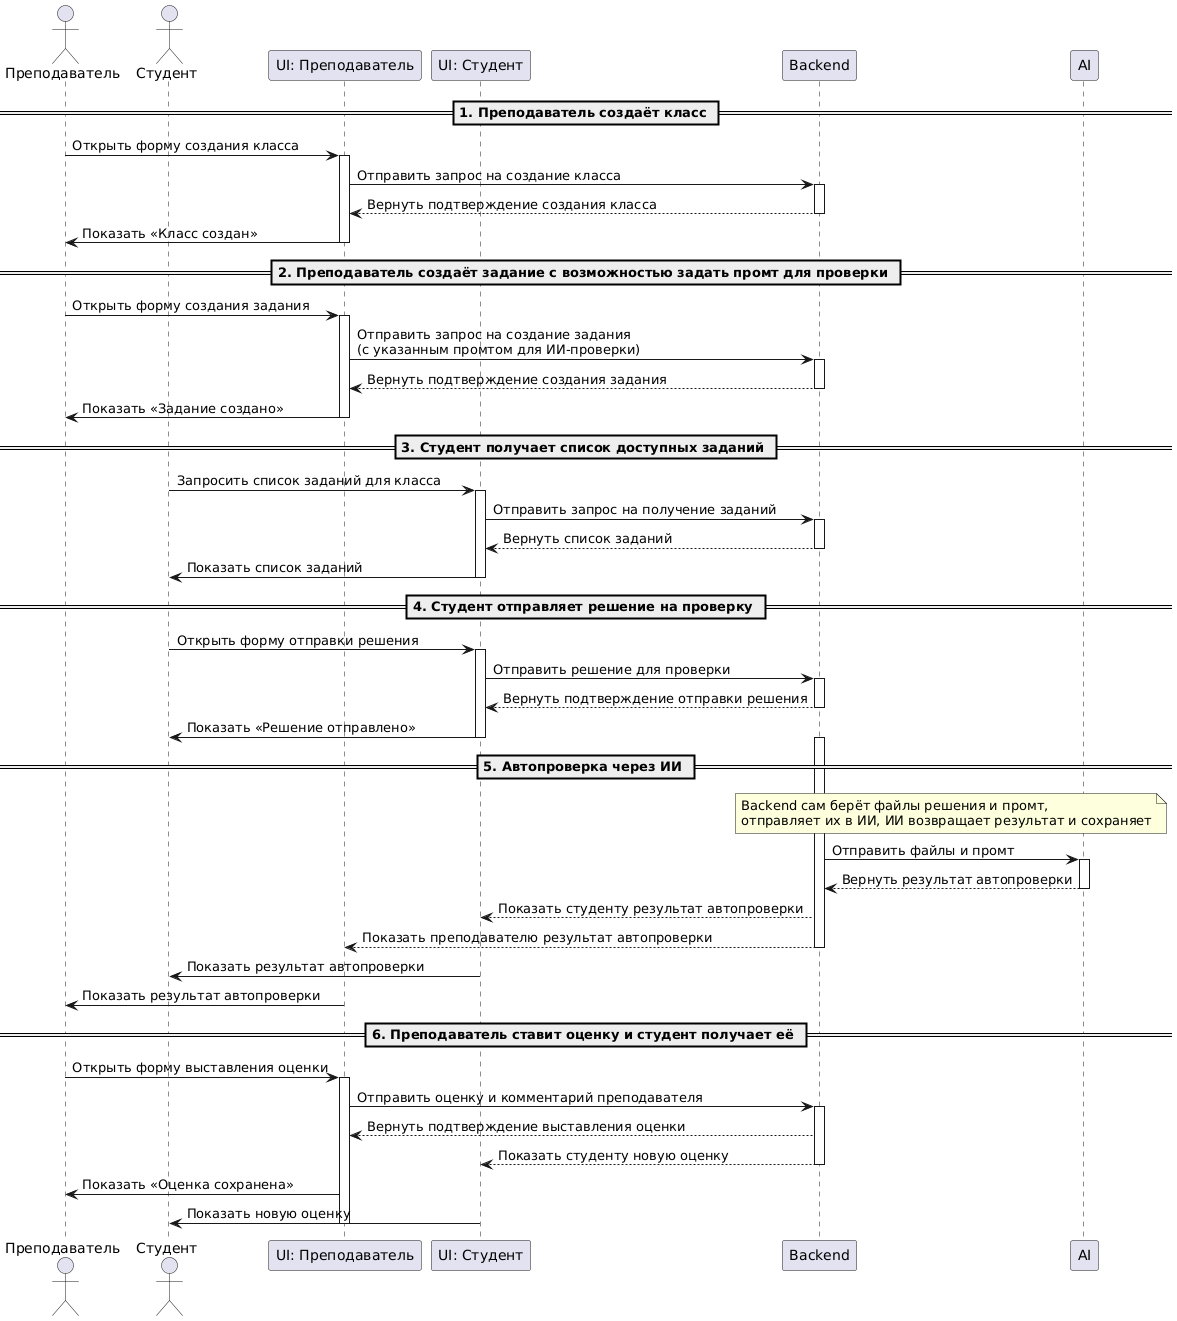
\includegraphics[width=0.9\textwidth]{static/diagrams/Classroom.png}
    \caption{Схема взаимодействия преподавателя, студента, UI, бэкенда и AI при работе с виртуальными классами}
    \label{fig:classroom-flow}
\end{figure}

На рисунке~\ref{fig:classroom-flow} можно выделить следующие ключевые этапы:

\begin{enumerate}
    \item \textbf{Преподаватель создаёт класс:}
    \begin{itemize}
        \item Преподаватель открывает форму создания класса в своем интерфейсе (UI: Преподаватель).
        \item UI отправляет запрос на бэкенд с данными нового класса.
        \item Бэкенд возвращает подтверждение успешного создания (например, ID нового класса).
        \item UI отображает преподавателю сообщение «Класс создан».
    \end{itemize}

    \item \textbf{Преподаватель создаёт задание с возможностью задать промт для AI-проверки:}
    \begin{itemize}
        \item Преподаватель переходит в форму создания задания, указывая вместе с условием текста задания промт для AI-проверки.
        \item UI отправляет запрос на бэкенд с данными задания и промтом.
        \item Бэкенд возвращает подтверждение успешного сохранения задания.
        \item UI отображает преподавателю сообщение «Задание создано».
    \end{itemize}

    \item \textbf{Студент получает список доступных заданий:}
    \begin{itemize}
        \item Студент открывает интерфейс (UI: Студент) и запрашивает список заданий для конкретного класса.
        \item UI отправляет запрос на бэкенд с ID класса.
        \item Бэкенд возвращает массив доступных заданий.
        \item UI отображает студенту список заданий.
    \end{itemize}

    \item \textbf{Студент отправляет решение на проверку:}
    \begin{itemize}
        \item Студент открывает форму отправки решения, выбирая конкретное задание.
        \item UI отправляет файлы решения и метаданные (например, ID задания, ID студента) на бэкенд.
        \item Бэкенд возвращает подтверждение успешной загрузки решения.
        \item UI отображает студенту сообщение «Решение отправлено».
    \end{itemize}

    \item \textbf{Автопроверка через AI:}
    \begin{itemize}
        \item Бэкенд получает файлы решения и ранее заданный промт к заданию.
        \item Бэкенд отправляет файлы и промт во внешний AI-сервис.
        \item AI-сервис выполняет анализ кода (например, проверку корректности, стилевых нарушений и т. д.) и возвращает результат вместе с комментариями.
        \item Бэкенд сохраняет результат автопроверки и передаёт его UI обоим ролям:
        \begin{itemize}
            \item UI Студента: отображается результат автопроверки (оценка AI, комментарии).
            \item UI Преподавателя: отображается результат автопроверки (для последующей ручной проверки и выставления итоговой оценки).
        \end{itemize}
    \end{itemize}

    \item \textbf{Преподаватель ставит оценку, и студент получает её:}
    \begin{itemize}
        \item Преподаватель открывает форму выставления оценки (UI: Преподаватель) для конкретного решения.
        \item UI отправляет в бэкенд оценку и комментарий преподавателя.
        \item Бэкенд сохраняет оценку, возвращает подтверждение сохранения.
        \item UI отображает преподавателю сообщение «Оценка сохранена», а UI Студента — обновлённую финальную оценку.
    \end{itemize}
\end{enumerate}

Таким образом, последовательная диаграмма на рисунке~\ref{fig:classroom-flow} демонстрирует весь цикл взаимодействий: от создания класса и задания преподавателем до получения студентом финальной оценки после автопроверки и ручного выставления оценки преподавателем.
